\documentclass[12pt,-letter paper]{article}
\usepackage{siunitx}
\usepackage{setspace}
\usepackage{gensymb}
\usepackage{xcolor}
\usepackage{caption}
%\usepackage{subcaption}
\doublespacing
\singlespacing
\usepackage[none]{hyphenat}
\usepackage{amssymb}
\usepackage{relsize}
\usepackage[cmex10]{amsmath}
\usepackage{mathtools}
\usepackage{amsmath}
\usepackage{commath}
\usepackage{amsthm}
\interdisplaylinepenalty=2500
%\savesymbol{iint}
\usepackage{txfonts}
%\restoresymbol{TXF}{iint}
\usepackage{wasysym}
\usepackage{amsthm}
\usepackage{mathrsfs}
\usepackage{txfonts}
\let\vec\mathbf{}
\usepackage{stfloats}
\usepackage{float}
\usepackage{cite}
\usepackage{cases}
\usepackage{subfig}
%\usepackage{xtab}
\usepackage{longtable}
\usepackage{multirow}
%\usepackage{algorithm}
\usepackage{amssymb}
%\usepackage{algpseudocode}
\usepackage{enumitem}
\usepackage{mathtools}
%\usepackage{eenrc}
%\usepackage[framemethod=tikz]{mdframed}
\usepackage{listings}
%\usepackage{listings}
\usepackage[latin1]{inputenc}
%%\usepackage{color}{   
%%\usepackage{lscape}
\usepackage{textcomp}
\usepackage{titling}
\usepackage{hyperref}
%\usepackage{fulbigskip}   
\usepackage{tikz}
\usepackage{graphicx}
\lstset{
  frame=single,
  breaklines=true
}
\let\vec\mathbf{}
\usepackage{enumitem}
\usepackage{graphicx}
\usepackage{siunitx}
\let\vec\mathbf{}
\usepackage{enumitem}
\usepackage{graphicx}
\usepackage{enumitem}
\usepackage{tfrupee}
\usepackage{amsmath}
\usepackage{amssymb}
\usepackage{mwe} % for blindtext and example-image-a in example
\usepackage{wrapfig}
\graphicspath{{figs/}}
\providecommand{\mydet}[1]{\ensuremath{\begin{vmatrix}#1\end{vmatrix}}}
\providecommand{\myvec}[1]{\ensuremath{\begin{bmatrix}#1\end{bmatrix}}}
\providecommand{\cbrak}[1]{\ensuremath{\left\{#1\right\}}}
\providecommand{\brak}[1]{\ensuremath{\left(#1\right)}}
\begin{document}
\begin{enumerate}
	\item Let $ABC$ be an acute-angled triangle  with $AB$ $\neq$ $AC$.The circle with diameter $BC$ intersects the sides $AB$ and $AC$ at $M$ and $N$ respectively.Denote  by $O$ the midpoint of the side $BC$.The bisector of the angles $<$$BAC$ and $<$$MON$ intersects at $R$.Prove that the circumcircles of the triangles $BMR$ and $CNR$ have a common point on the side $BC$ 
	\item Find all polynomials of $f$ with real coefficient such that for all reals $a,b,c$ such that $ab+bc+ca=0$ We have the following relations \\ $f$ $(a-b)$+$f$ $(b-c)$ + $f$ $(c-a)$ = $2f$ $(a+b+c)$
	\item Define a "hook" to be a figure made up of six unit squares as shown below in the picture,or any of the figures obtained by applying rotations and reflections to this figure. 
\begin{figure}[!ht]
  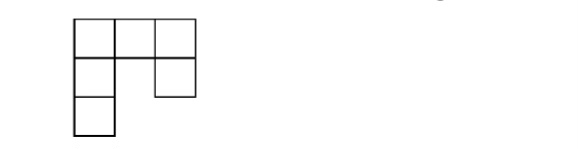
\includegraphics[width=\columnwidth]   {./img2.jpg}
                \end{figure}
Determine all mxn rectangles that can be covered without gaps and without overlaps with hooks such that\\
$\bullet$ the rectangle is covered without gaps and without overlaps\\
$\bullet$ no part of a hook covers area outside the rectangle.
	\item Let n $\geq$ 3 be an integer.Let $t_1$,$t_2$......$t_n$ be positive real numbers such that \\ $n^{2}+1>\brak{t_1,t_2......t_n}$  $\brak{\frac{1}{t_1}+\frac{1}{t_2}+.......\frac{1}{t_n}}$ 
	\item In a convex quadrilateral ABCD the diagonal BD does not bisect the angles ABC and CDA.The point P lies inside ABCD and satisfies 
\begin{align*}
\angle{PBC}=\angle{DBA} and \angle{PDC}=\angle{BDA}.
\end{align*}
Prove that ABCD is a cyclic quadrilateral if and only if AP=CP
	\item We call a positive integer alternating if every two consecutive digits in its decimal representation are of different parity.Find all positive integers $n$ such that $n$ has a multiple which is alternating 
	 

\end{enumerate}
\end{document}
